% Options for packages loaded elsewhere
\PassOptionsToPackage{unicode}{hyperref}
\PassOptionsToPackage{hyphens}{url}
%
\documentclass[
]{article}
\usepackage{amsmath,amssymb}
\usepackage{lmodern}
\usepackage{iftex}
\ifPDFTeX
  \usepackage[T1]{fontenc}
  \usepackage[utf8]{inputenc}
  \usepackage{textcomp} % provide euro and other symbols
\else % if luatex or xetex
  \usepackage{unicode-math}
  \defaultfontfeatures{Scale=MatchLowercase}
  \defaultfontfeatures[\rmfamily]{Ligatures=TeX,Scale=1}
\fi
% Use upquote if available, for straight quotes in verbatim environments
\IfFileExists{upquote.sty}{\usepackage{upquote}}{}
\IfFileExists{microtype.sty}{% use microtype if available
  \usepackage[]{microtype}
  \UseMicrotypeSet[protrusion]{basicmath} % disable protrusion for tt fonts
}{}
\makeatletter
\@ifundefined{KOMAClassName}{% if non-KOMA class
  \IfFileExists{parskip.sty}{%
    \usepackage{parskip}
  }{% else
    \setlength{\parindent}{0pt}
    \setlength{\parskip}{6pt plus 2pt minus 1pt}}
}{% if KOMA class
  \KOMAoptions{parskip=half}}
\makeatother
\usepackage{xcolor}
\IfFileExists{xurl.sty}{\usepackage{xurl}}{} % add URL line breaks if available
\IfFileExists{bookmark.sty}{\usepackage{bookmark}}{\usepackage{hyperref}}
\hypersetup{
  hidelinks,
  pdfcreator={LaTeX via pandoc}}
\urlstyle{same} % disable monospaced font for URLs
\usepackage{graphicx}
\makeatletter
\def\maxwidth{\ifdim\Gin@nat@width>\linewidth\linewidth\else\Gin@nat@width\fi}
\def\maxheight{\ifdim\Gin@nat@height>\textheight\textheight\else\Gin@nat@height\fi}
\makeatother
% Scale images if necessary, so that they will not overflow the page
% margins by default, and it is still possible to overwrite the defaults
% using explicit options in \includegraphics[width, height, ...]{}
\setkeys{Gin}{width=\maxwidth,height=\maxheight,keepaspectratio}
% Set default figure placement to htbp
\makeatletter
\def\fps@figure{htbp}
\makeatother
\setlength{\emergencystretch}{3em} % prevent overfull lines
\providecommand{\tightlist}{%
  \setlength{\itemsep}{0pt}\setlength{\parskip}{0pt}}
\setcounter{secnumdepth}{-\maxdimen} % remove section numbering
\ifLuaTeX
  \usepackage{selnolig}  % disable illegal ligatures
\fi

\author{}
\date{}

\begin{document}

\hypertarget{correction}{%
\section{Correction}\label{correction}}

\hypertarget{exercice-1-la-croix-keynuxe9sienne}{%
\subsection{Exercice 1: la croix
keynésienne}\label{exercice-1-la-croix-keynuxe9sienne}}

On considère une économie simplifiée où l'équilibre dépend de la
production totale \(Y\) et du taux d'intérêt \emph{réel} \(r\). Il
s'agit d'un modèle de court terme de sorte que l'on omet les indices
temporels. Tout au long de cet exercice, nous supposons que les prix
sont fixes (nous faisons donc abstraction de l'offre agrégée). Les
composantes de la demande agrégée sont:

\begin{itemize}
\tightlist
\item
  la consommation totale des ménages: \(C=C(Y,r)\)
\item
  l'investissement total des entreprises: \(I=I(r)\)
\item
  les dépenses gouvernementales \(G\) choisies de manière exogène par le
  gouvernement \(G\)
\end{itemize}

\hypertarget{la-croix-keynuxe9sienne}{%
\subsubsection{La croix keynésienne}\label{la-croix-keynuxe9sienne}}

\begin{enumerate}
\def\labelenumi{\arabic{enumi}.}
\tightlist
\item
  \textbf{Écrire la relation définissant l'équilibre sur le marché des
  biens à l'état stationnaire \((\overline{Y},\overline{r})\). Justifier
  brièvement, sans calcul, le signe des dérivées
  \(C^{\prime}_Y(\overline{Y},\overline{r})\),
  \(C^{\prime}_r(\overline{Y},\overline{r})\) et
  \(I^{\prime}(\overline{r})\).}
\end{enumerate}

Nous analysons la détermination de l'équilibre au moyen d'un graphique
(diagramme à 45 degrés, aussi appelé croix keynésienne): la demande est
représentée sur l'axe vertical et la production est représentée sur
l'axe horizontal. La production d'équilibre est donnée par l'égalité
entre la production et la demande.

\begin{figure}
\centering
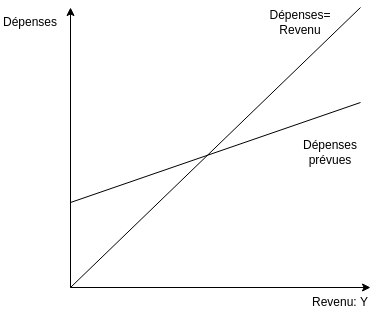
\includegraphics{cross.png}
\caption{Croix Keynesienne}
\end{figure}

\begin{enumerate}
\def\labelenumi{\arabic{enumi}.}
\setcounter{enumi}{1}
\item
  \textbf{On suppose maintenant que le gouvernement augmente ses
  dépenses d'une quantité infinitésimale \(\Delta G\) sans effet sur les
  taux d'intérêt. Quelle est l'augmentation \(\Delta Y\) de la
  production d'équilibre ? Calculer le multiplicateur fiscal
  \(\frac{\Delta Y}{\Delta G}\). Représenter cette augmentation sur le
  diagramme à 45 degrés.}
\item
  \textbf{Dans la question précédente, on n'a pas précisé comment était
  financée la dépense supplémentaire (peut-être par un emprunt remboursé
  dans le futur). On suppose maintenant que le gouvernement impose une
  taxe forfaitaire \(\Delta T\) sur le revenu des ménages pour financer
  ses dépenses (\(\Delta T=\Delta G\)). Avec ces taxes, la consommation
  totale des ménages est une fonction du revenu disponible
  \(C=C(Y-\Delta T, r)\). De combien augmente la production d'équilibre
  et quel est le nouveau multiplicateur fiscal? Comment interpréter le
  résultat?}
\item
  \textbf{Calculer et représenter sur un graphe du même type l'effet
  d'une baisse des taux d'intérêt nominaux en supposant que les prix
  sont fixes à court terme.}
\end{enumerate}

\hypertarget{agents-huxe9tuxe9roguxe8nes}{%
\subsubsection{Agents hétérogènes}\label{agents-huxe9tuxe9roguxe8nes}}

On suppose maintenant que les agents sont répartis en 2 groupes: les
agents de type \(H\) (hand-to-mouth), pour une fraction \(\lambda\), et
les agents de type \(S\) (savers) pour une fraction \(1-\lambda\). Les
agents \(H\) n'ont pas accès aux marchés financiers et tous leurs
revenus proviennent du travail. Les agents \(S\) (pour savers) peuvent
lisser leur consommation par l'epargne. Ces derniers recoivent en plus
de leur travail, les revenus du capital et les profits des firmes. Les
différent revenus seront définis plus bas.

\begin{enumerate}
\def\labelenumi{\arabic{enumi}.}
\setcounter{enumi}{4}
\item
  \textbf{On suppose que les fonctions de consommation des deux groupes
  sont données par:} \begin{align}
  C^H(Y^H,r) & = & c^H_0 & + c^H_Y (Y_H - \overline{Y_H}) &  & \;\text{avec} & 1\approx c^1_H<1\\
  C^S(Y^S,r) & = & c^S_0 & + c^S_Y (Y_S - \overline{Y_S}) & + c^S_r (r-\overline{r}) & \;\text{avec} & 0<c_1^S\approx 0 
  \end{align} \textbf{où \(\overline{Y_H}\) (resp \(\overline{Y_S}\))
  est le revenu perçu à l'équilibre par les agents \(H\) (resp \(S\))}
\item
  \textbf{Justifier \emph{intuitivement} les hypothèses sur \(c^H_Y\) et
  \(c^S_Y\). A-t-on assez d'infomations pour calculer la propension
  marginale à consommer agrégée\footnote{La propension marginale à
    consommer agrégée est l'augmentation de la consommation prévue
    totale, lorsque le revenu total augmente d'une unité.} comme dans la
  question 1?}
\end{enumerate}

On fait maintenant les hypothèses suivantes sur la répartition du revenu
total:

\begin{itemize}
\tightlist
\item
  tous les agents travaillent au même salaire \(W\)
\item
  une fraction \(\alpha_L\) des revenus totaux revient aux travailleurs,
  une fraction \(\alpha_K\) aux détenteurs du capital et une fraction
  \(\alpha_\pi\) est payée sous forme de profits au détenteurs des
  firmes. On a bien sûr \(\alpha_L + \alpha_K + \alpha_\pi=1\)
\item
  le gouvernements taxe les profits et les revenus du capital à un taux
  \(\tau\), pour les redistribuer aux agents \(H\)
\end{itemize}

\begin{enumerate}
\def\labelenumi{\arabic{enumi}.}
\setcounter{enumi}{6}
\tightlist
\item
  \textbf{Calculer la propension marginale à consommer agrégée.
  Peut-elle être plus grande que 1? Quel est le multiplicateur fiscal.}
\end{enumerate}

\end{document}
